\chapter{Моделирование в среде Matlab/Simulink}
\label{ch:chap3}

В среде Matlab/Simulink была создана модель квадрокоптера,
основанная на синтезированных уравнениях.
Было проведено моделирование квадрокоптера в задаче слежения за траекторией
с разными регуляторами. Использовались две траектории: `восьмерка' и `куб'.

В качестве регуляторов использовались LQR по линеаризованной модели,
двухконтурный LQR с линеаризацией обратной связью и Nonlinear MPC.

Графики результатов представлены ниже в этой главе, также были построены метрики
для оценки качества переходных процессов и результаты приведены в 

% \begin{figure}[ht]
%     \centering
%     \includegraphics[width=0.8 \textwidth]{Simulink-model.png}
%     \caption{Модель квадрокоптера в Simulink}
%     \label{}
% \end{figure}

\section{Графики моделирования}

\begin{figure}[ht]
    \centering
    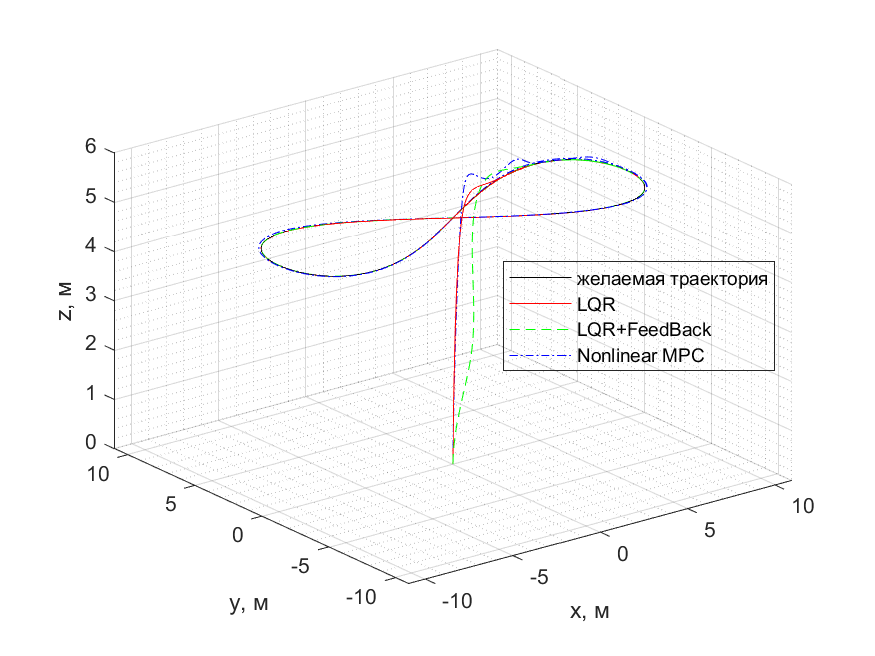
\includegraphics[width=0.8 \textwidth]{3d/eight_no_ressist.png}
    \caption{Моделирование квадрокоптера в трёхмерном пространстве с отсутствующим внешним сопротивлением}
    \label{}
\end{figure}


\begin{figure}[ht]
    \centering
    \includegraphics[width=0.8 \textwidth]{MPC_1/error_position_eight_no_ressist.png}
    \caption{График ошибок положения квадрокоптера в трёхмерном пространстве с отсутствующим внешним сопротивлением при использовании Nonlinear MPC}
    \label{}
\end{figure}

\begin{figure}[ht]
	\centering
\hspace*{\fill}%
	\begin{subfigure}[b]{0.49\textwidth}
        \centering
		\includegraphics[height=9cm,keepaspectratio]{LQR_1/error_position_eight_no_ressist.png}
		\caption{}
		\label{fig:tiger1}
	\end{subfigure}
\hfill
	\begin{subfigure}[b]{0.49\textwidth}
        \centering
		\includegraphics[height=9cm,keepaspectratio]{LQR_2/error_position_eight_no_ressist.png}
        \caption{}
		\label{fig:tiger2}
	\end{subfigure}
\hspace*{\fill}%
	\caption{Графики ошибок положения квадрокоптера в трёхмерном пространстве с отсутствующим внешним сопротивлением. На рисунке (а) LQR по линеаризованной модели. На рисунке (б) двухконтурный LQR с линеаризацией обратной связью}
	\label{fig:tiger}
\end{figure}

\newpage

\begin{figure}[ht]
    \centering
    \includegraphics[width=0.8 \textwidth]{MPC_1/orientation_eight_no_ressist.png}
    \caption{График ориентации квадрокоптера с отсутствующим внешним сопротивлением при использовании Nonlinear MPC}
    \label{}
\end{figure}

\begin{figure}[ht]
	\centering
\hspace*{\fill}%
	\begin{subfigure}[b]{0.49\textwidth}
        \centering
		\includegraphics[height=9cm,keepaspectratio]{LQR_1/orientation_eight_no_ressist.png}
		\caption{}
		\label{fig:tiger1}
	\end{subfigure}
\hfill
	\begin{subfigure}[b]{0.49\textwidth}
        \centering
		\includegraphics[height=9cm,keepaspectratio]{LQR_2/orientation_eight_no_ressist.png}
        \caption{}
		\label{fig:tiger2}
	\end{subfigure}
\hspace*{\fill}%
	\caption{Графики ориентации квадрокоптера с отсутствующим внешним сопротивлением. На рисунке (а) LQR по линеаризованной модели. На рисунке (б) двухконтурный LQR с линеаризацией обратной связью}
	\label{fig:tiger}
\end{figure}

\newpage

\begin{figure}[ht]
    \centering
    \includegraphics[width=0.8 \textwidth]{MPC_1/control_inputs_eight_no_ressist.png}
    \caption{График управления квадрокоптера с отсутствующим внешним сопротивлением при использовании Nonlinear MPC}
    \label{}
\end{figure}

\begin{figure}[ht]
	\centering
\hspace*{\fill}%
	\begin{subfigure}[b]{0.49\textwidth}
        \centering
		\includegraphics[height=9cm,keepaspectratio]{LQR_1/control_inputs_eight_no_ressist.png}
		\caption{}
		\label{fig:tiger1}
	\end{subfigure}
\hfill
	\begin{subfigure}[b]{0.49\textwidth}
        \centering
		\includegraphics[height=9cm,keepaspectratio]{LQR_2/control_inputs_eight_no_ressist.png}
        \caption{}
		\label{fig:tiger2}
	\end{subfigure}
\hspace*{\fill}%
	\caption{Графики управления квадрокоптера с отсутствующим внешним сопротивлением. На рисунке (а) LQR по линеаризованной модели. На рисунке (б) двухконтурный LQR с линеаризацией обратной связью}
	\label{fig:tiger}
\end{figure}

%%%%%%%%%%%%%%%%%%%%%%%%%%%%%%%%%%%%%%%% RESIST EIGHT
\newpage 

\begin{figure}[ht]
    \centering
    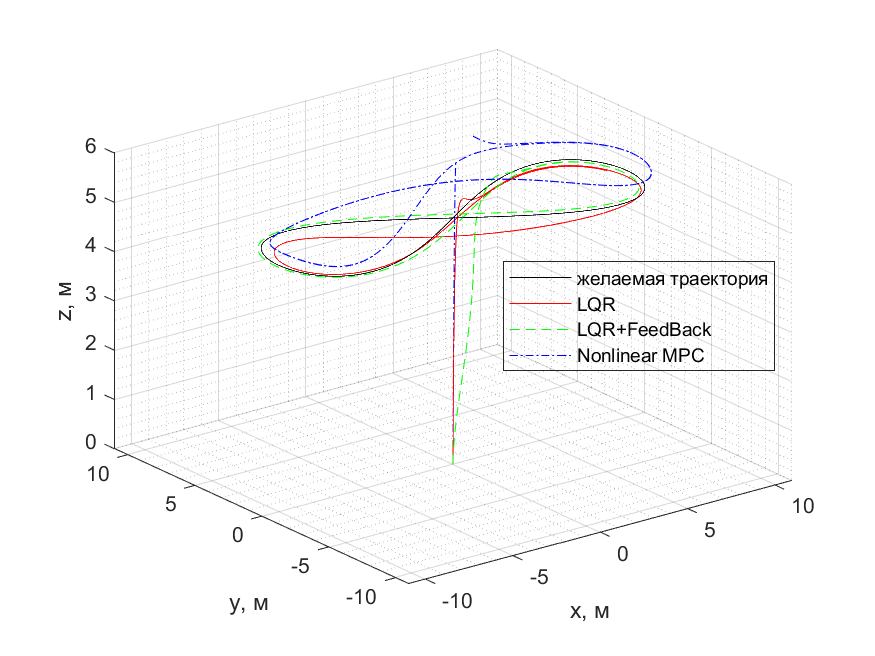
\includegraphics[width=0.8 \textwidth]{3d/eight_normal_resist.png}
    \caption{Моделирование квадрокоптера в трёхмерном пространстве при наличии внешнего сопротивления}
    \label{}
\end{figure}


\begin{figure}[ht]
    \centering
    \includegraphics[width=0.8 \textwidth]{MPC_1/error_position_eight_normal_resist.png}
    \caption{График ошибок положения квадрокоптера в трёхмерном пространстве при наличии внешнего сопротивления при использовании Nonlinear MPC}
    \label{}
\end{figure}

\begin{figure}[ht]
	\centering
\hspace*{\fill}%
	\begin{subfigure}[b]{0.49\textwidth}
        \centering
		\includegraphics[height=9cm,keepaspectratio]{LQR_1/error_position_eight_normal_resist.png}
		\caption{}
		\label{fig:tiger1}
	\end{subfigure}
\hfill
	\begin{subfigure}[b]{0.49\textwidth}
        \centering
		\includegraphics[height=9cm,keepaspectratio]{LQR_2/error_position_eight_normal_resist.png}
        \caption{}
		\label{fig:tiger2}
	\end{subfigure}
\hspace*{\fill}%
	\caption{Графики ошибок положения квадрокоптера в трёхмерном пространстве при наличии внешнего сопротивления. На рисунке (а) LQR по линеаризованной модели. На рисунке (б) двухконтурный LQR с линеаризацией обратной связью}
	\label{fig:tiger}
\end{figure}

\newpage

\begin{figure}[ht]
    \centering
    \includegraphics[width=0.8 \textwidth]{MPC_1/orientation_eight_normal_resist.png}
    \caption{График ориентации квадрокоптера при наличии внешнего сопротивления при использовании Nonlinear MPC}
    \label{}
\end{figure}

\begin{figure}[ht]
	\centering
\hspace*{\fill}%
	\begin{subfigure}[b]{0.49\textwidth}
        \centering
		\includegraphics[height=9cm,keepaspectratio]{LQR_1/orientation_eight_normal_resist.png}
		\caption{}
		\label{fig:tiger1}
	\end{subfigure}
\hfill
	\begin{subfigure}[b]{0.49\textwidth}
        \centering
		\includegraphics[height=9cm,keepaspectratio]{LQR_2/orientation_eight_normal_resist.png}
        \caption{}
		\label{fig:tiger2}
	\end{subfigure}
\hspace*{\fill}%
	\caption{Графики ориентации квадрокоптера при наличии внешнего сопротивления. На рисунке (а) LQR по линеаризованной модели. На рисунке (б) двухконтурный LQR с линеаризацией обратной связью}
	\label{fig:tiger}
\end{figure}

\newpage

\begin{figure}[ht]
    \centering
    \includegraphics[width=0.8 \textwidth]{MPC_1/control_inputs_eight_normal_resist.png}
    \caption{График управления квадрокоптера при наличии внешнего сопротивления при использовании Nonlinear MPC}
    \label{}
\end{figure}

\begin{figure}[ht]
	\centering
\hspace*{\fill}%
	\begin{subfigure}[b]{0.49\textwidth}
        \centering
		\includegraphics[height=9cm,keepaspectratio]{LQR_1/control_inputs_eight_normal_resist.png}
		\caption{}
		\label{fig:tiger1}
	\end{subfigure}
\hfill
	\begin{subfigure}[b]{0.49\textwidth}
        \centering
		\includegraphics[height=9cm,keepaspectratio]{LQR_2/control_inputs_eight_normal_resist.png}
        \caption{}
		\label{fig:tiger2}
	\end{subfigure}
\hspace*{\fill}%
	\caption{Графики управления квадрокоптера при наличии внешнего сопротивления. На рисунке (а) LQR по линеаризованной модели. На рисунке (б) двухконтурный LQR с линеаризацией обратной связью}
	\label{fig:tiger}
\end{figure}


%%%%%%%%%%%%%%%%%%%%%%%%%%%%% CUBE

\begin{figure}[ht]
    \centering
    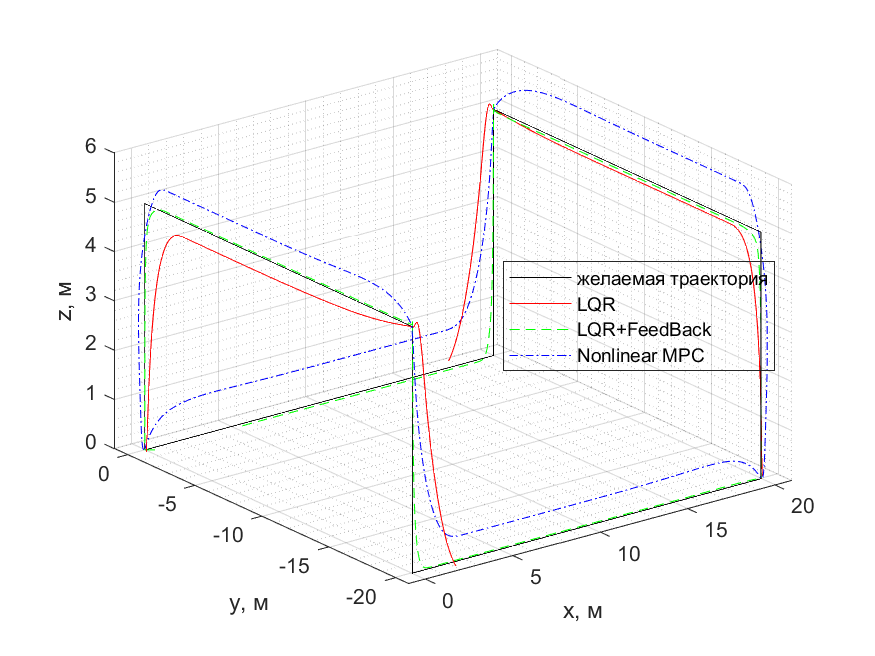
\includegraphics[width=0.8 \textwidth]{3d/fig_normal_resist.png}
    \caption{Моделирование квадрокоптера в трёхмерном пространстве при наличии внешнего сопротивления}
    \label{}
\end{figure}



\begin{figure}[ht]
    \centering
    \includegraphics[width=0.8 \textwidth]{MPC_1/error_position_fig_normal_resist.png}
    \caption{График ошибок положения квадрокоптера в трёхмерном пространстве при наличии внешнего сопротивления при использовании Nonlinear MPC}
    \label{}
\end{figure}

\begin{figure}[ht]
	\centering
\hspace*{\fill}%
	\begin{subfigure}[b]{0.49\textwidth}
        \centering
		\includegraphics[height=9cm,keepaspectratio]{LQR_1/error_position_fig_normal_resist.png}
		\caption{}
		\label{fig:tiger1}
	\end{subfigure}
\hfill
	\begin{subfigure}[b]{0.49\textwidth}
        \centering
		\includegraphics[height=9cm,keepaspectratio]{LQR_2/error_position_fig_normal_resist.png}
        \caption{}
		\label{fig:tiger2}
	\end{subfigure}
\hspace*{\fill}%
	\caption{Графики ошибок положения квадрокоптера в трёхмерном пространстве при наличии внешнего сопротивления. На рисунке (а) LQR по линеаризованной модели. На рисунке (б) двухконтурный LQR с линеаризацией обратной связью}
	\label{fig:tiger}
\end{figure}

\newpage

\begin{figure}[ht]
    \centering
    \includegraphics[width=0.8 \textwidth]{MPC_1/orientation_fig_normal_resist.png}
    \caption{График ориентации квадрокоптера при наличии внешнего сопротивления при использовании Nonlinear MPC}
    \label{}
\end{figure}

\begin{figure}[ht]
	\centering
\hspace*{\fill}%
	\begin{subfigure}[b]{0.49\textwidth}
        \centering
		\includegraphics[height=9cm,keepaspectratio]{LQR_1/orientation_fig_normal_resist.png}
		\caption{}
		\label{fig:tiger1}
	\end{subfigure}
\hfill
	\begin{subfigure}[b]{0.49\textwidth}
        \centering
		\includegraphics[height=9cm,keepaspectratio]{LQR_2/orientation_fig_normal_resist.png}
        \caption{}
		\label{fig:tiger2}
	\end{subfigure}
\hspace*{\fill}%
	\caption{Графики ориентации квадрокоптера при наличии внешнего сопротивления. На рисунке (а) LQR по линеаризованной модели. На рисунке (б) двухконтурный LQR с линеаризацией обратной связью}
	\label{fig:tiger}
\end{figure}

\newpage

\begin{figure}[ht]
    \centering
    \includegraphics[width=0.8 \textwidth]{MPC_1/control_inputs_fig_normal_resist.png}
    \caption{График управления квадрокоптера при наличии внешнего сопротивления при использовании Nonlinear MPC}
    \label{}
\end{figure}

\begin{figure}[ht]
	\centering
\hspace*{\fill}%
	\begin{subfigure}[b]{0.49\textwidth}
        \centering
		\includegraphics[height=9cm,keepaspectratio]{LQR_1/control_inputs_fig_normal_resist.png}
		\caption{}
		\label{fig:tiger1}
	\end{subfigure}
\hfill
	\begin{subfigure}[b]{0.49\textwidth}
        \centering
		\includegraphics[height=9cm,keepaspectratio]{LQR_2/control_inputs_fig_normal_resist.png}
        \caption{}
		\label{fig:tiger2}
	\end{subfigure}
\hspace*{\fill}%
	\caption{Графики управления квадрокоптера при наличии внешнего сопротивления. На рисунке (а) LQR по линеаризованной модели. На рисунке (б) двухконтурный LQR с линеаризацией обратной связью}
	\label{fig:tiger}
\end{figure}


\section{Метрики качества переходных процессов}

\begin{table}[ht]
    \caption{Метрики качества переходных процессов на траектории `восьмерка'}
    \label{tab:t1}
    \centering
    \begin{tabular}{l c c c c}
    \hline
    Система управления  & {J} & {\(RMSE x\)} & {\(RMSE y\)} & {\(RMSE z\)}  \\ \hline
    LQR(без сопротивления) & 2577.27 & 1.141 & 0.739 & 0.863  \\
    LQR(малое сопротивление) & 2696.34 & 1.230 & 0.789 & 0.862 \\
    LQR(большое сопротивление) & 4520.52 & 2.108 & 1.230 & 0.880 \\
    LQR+FB(без сопротивления) & 1955.86 & 0.470 & 0.324 & 0.798\\
    LQR+FB(малое сопротивление) & 1965.11 & 0.486 & 0.335 & 0.798\\
    LQR+FB(большое сопротивление) & 2321.46 & 0.653 & 0.425 & 0.787  \\
    MPC(без сопротивления) & 2797.40 & 0.463 & 0.305 & 0.501\\
    MPC(малое сопротивление) & 2852.15 & 0.524 & 0.344 & 0.495   \\
    MPC(большое сопротивление) & 4127.30 & 1.081 & 0.772 & 1.033 \\ \hline
    \end{tabular}
\end{table}


% \begin{table}[ht]
%     \caption{Метрики качества переходных процессов на траектории `восьмерка'}
%     \label{tab:t1}
%     \centering
%     \begin{tabular}{l c c c c}
%     \hline
%     Система управления & {RMSE} & {\(RMSE x\)} & {\(RMSE y\)} & {\(RMSE z\)}  \\ \hline
%     LQR(Без сопротивления) & 0.914 & 1.141 & 0.739 & 0.863  \\
%     LQR(При наличии сопротивления) & 1.406 & 2.108 & 1.230 & 0.880 \\
%     LQR+FB(Без сопротивления) & 0.510 & 0.470 & 0.324 & 0.798\\
%     LQR+FB(При наличии сопротивления) & 0.622 & 0.653 & 0.425 & 0.787  \\
%     MPC(Без сопротивления) & 0.423 & 0.463 & 0.305 & 0.501\\
%     MPC(При наличии сопротивления) & 0.962 & 1.081 & 0.772 & 1.033 \\ \hline
%     \end{tabular}
% \end{table}

\begin{table}[ht]
    \caption{Метрики качества переходных процессов на траектории `куб'}
    \label{tab:t2}
    \centering
    \begin{tabular}{l c c c c}
    \hline
    Система управления & J & \(RMSE x\) & \(RMSE y\) & \(RMSE z\)  \\ \hline
    LQR(без сопротивления) & 3724.78 & 0.939 & 0.931 & 0.502  \\
    LQR(малое сопротивление) & 3895.01 & 1.004 & 1.002 & 0.501\\
    LQR(большое сопротивление) & 6597.09 & 1.689 & 1.718 & 0.542 \\
    LQR+FB(без сопротивления) & 3094.73 & 0.519 & 0.514 & 0.637\\
    LQR+FB(малое сопротивление) & 3121.09 & 0.537 & 0.537 & 0.647\\
    LQR+FB(большое сопротивление) & 3877.34 & 0.758 & 0.756 & 0.633  \\
    MPC(без сопротивления) & 2576.46& 0.274 & 0.274 & 0.107\\
    MPC(малое сопротивление) & 2607.05 & 0.323 & 0.321 & 0.106   \\
    MPC(большое сопротивление) & 4122.27 & 0.973 & 0.948 & 0.493 \\ \hline
    \end{tabular}
\end{table}

Как видно из таблиц \ref{tab:t1} и \ref{tab:t2},
MPC регулятор показал лучшие результаты при моделировании без 
возмущений. Однако при наличии сильных возмущений лучше 
всего себя показал LQR регулятор с линеаризацией по обратной связью.



\endinput